\justifying
\NSFCBodyText

\subsubsection{与本项目相关的研究工作积累}

申请人长期从事机器学习、深度学习、多源信息融合与模型训练研究，在研究问题凝练、表征与模型设计、实验组织、结果分析和软件实现方面积累了经验。这些工作尚不是中文预训练语料质量机制的专属先导研究，但可从三个方面支撑本项目：异质信息的分层表示、匹配与解耦经验，有助于区分静态质量表征、结构完整性与模型熟悉度；条件校准、状态空间推理和多层表征研究，有助于分析处理前状态、训练轨迹和能力终点之间的关系；数据治理、模型训练、自动实验、版本管理和统计评价能力，则可支撑多处理臂、成对随机种子与冻结协议的可复现实施。

在代表性工作中，申请人作为通讯作者完成了跨模态检索研究“Feature Fusion Mamba Hashing via Decoupling for Cross-Modal Retrieval”（\emph{IEEE Signal Processing Letters}, 2026, DOI: 10.1109/LSP.2026.3652952），负责研究构思、方法设计、实验指导、结果分析及论文撰写与修改。该工作形成了对耦合因素进行分解并通过对照实验验证的研究经验，可迁移到本项目“评分相近但生成机制不同”的变量拆分。申请人作为通讯作者完成了遥感视觉问答研究“RSHR+: Progressive Question-Conditioned Visual Calibration and Structured State-Space Reasoning for Remote Sensing Visual Question Answering”（\emph{Expert Systems with Applications}, 2026, 328: 132953, DOI: 10.1016/j.eswa.2026.132953），积累了条件校准、结构化状态建模和复杂评价组织经验。申请人作为第一作者、通讯作者完成了“Knowledge-Aware Image Understanding with Multi-Level Visual Representation Enhancement for Visual Question Answering”（\emph{Machine Learning}, 2024, 113(6): 3789--3805, DOI: 10.1007/s10994-023-06426-6），形成了多层表示与知识相关能力评价的研究基础。

\paragraph{公开数据上的结构操纵预实验。}为先检查数据可得性、扰动管道和恢复对照，申请人下载了\href{https://huggingface.co/datasets/CASIA-LM/ChineseWebText2.0}{ChineseWebText2.0}公开测试集（数据卡声明 Apache-2.0；原文件 1,000 条，文件哈希已归档）。按文本长度 400--600 字、发布方质量分不低于 0.35 且毒性标签为 0 筛得 122 条；固定随机种子 20270906，以 30 条选定扰动强度，其余 50 条作独立评估。预实验对每条文本生成简体归一化原文、语义/顺序不变的繁体字形变体、字符块置换扰动、依索引精确逆变换的恢复文本，以及从同一破损前体出发但不执行逆变换的 sham 文本。

在固定版本的\href{https://huggingface.co/Qwen/Qwen2.5-0.5B}{Qwen2.5-0.5B}（Apache-2.0）上，标定集从 4--128 字的候选块宽中选定 128 字，随后冻结参数。在 50 条评估样本上，原文、完整字形变体、结构扰动、精确恢复和 sham 的中位 causal-LM loss 分别为 3.101、3.049、3.379、3.101 和 3.368，五组均未触发 1,024-token 截断。扰动相对原文的成对中位差为 0.211（95\% bootstrap CI: 0.180--0.276）；精确恢复率为 100\% 且恢复后损失与原文完全一致，sham 非恢复率为 100\%。字符三元语言模型在另一评估集上得到相同方向，表明该方向不依赖单一评分器。

该预实验只证明公开数据/模型可访问、扰动可计算且逆操作可核查，不等同于继续预训练、能力终点或因果机制验证。扰动与字形变体虽有 0.66 的直方图重叠率，但成对中位差仍为 0.303（95\% bootstrap CI: 0.220--0.360），不支持静态评分等价。而且繁简转换改变了 token 数。因此，正式研究仍须用段落错序/连接破坏替代固定字符块，完成双人语体和语义保持审计，并严格匹配 token 与 packing。上述代表成果仍只作为方法论与研究组织能力证据；本申请不主张已有性能提升或机制验证。

\begin{figure}[htbp]
  \centering
  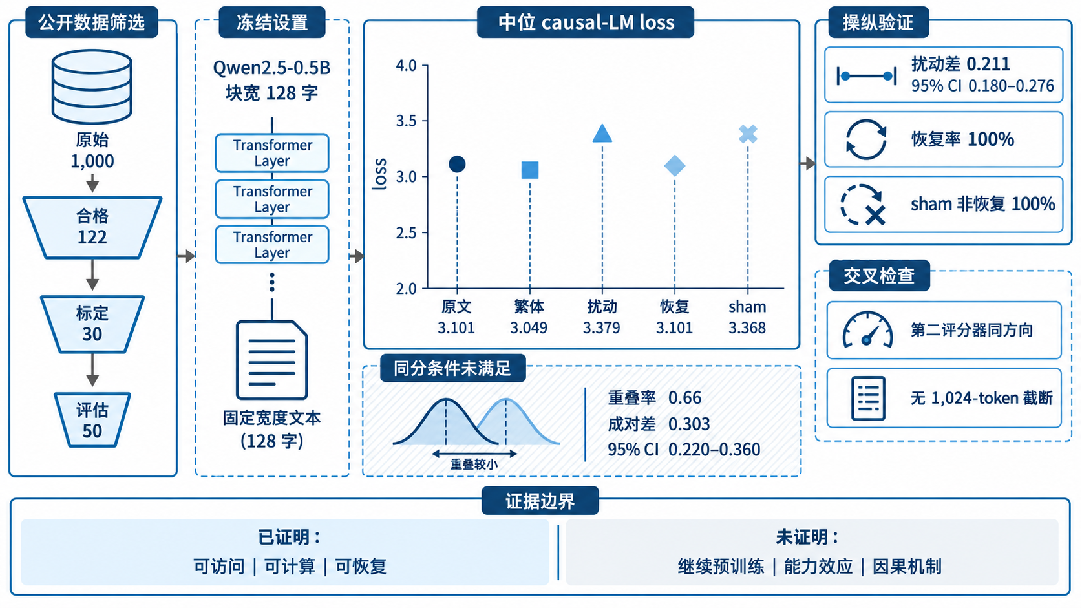
\includegraphics[width=0.98\linewidth]{figures/F13-preexperiment.pdf}
  \caption{公开数据结构操纵预实验流程、结果与证据边界}
  \label{fig:preexperiment}
\end{figure}

\subsubsection{已取得的研究工作成绩}

申请人已取得的相关成绩主要表现为独立组织机器学习研究、指导实验实施和完成同行评议成果的能力。前述三项代表性论文均已核验题录与作者贡献，其中两项由申请人担任通讯作者，一项由申请人担任第一作者兼通讯作者。它们分别覆盖解耦式表征融合、问题条件校准与结构化推理、多层知识相关表征，能够为本项目的路径拆分、状态条件分析和多层能力评价提供经验支撑。

申请人主持自治区高校基本科研业务费培育类项目和政企数字化知识库横向课题，并参与国家自然科学基金地区项目等科研任务，具备项目计划、数据整理、模型研究和成果组织经验。现有在研项目的题目、经费、执行期和与本申请的关系在“正在承担的科研项目情况”中如实列示；本项目不把其他项目的论文、数据或代码自动归入当前申请，也不把参与项目的总经费视为本项目可支配条件。

在科研工程条件方面，申请人已具备 Linux、Python、深度学习框架、Git 和 LaTeX 等工具链使用基础，能够建立数据版本、训练配置、随机种子、checkpoint、评测版本和统计输出之间的追踪关系。这些条件能够支撑运行记录清单（run manifest）、双来源冻结协议和失败结果保留。上述预实验已形成公开数据版本清单、确定性扰动/恢复/sham 脚本和静态评分记录；正式语料索引、双人中文语体标注、六臂反事实生成器、继续预训练和动力学测量代码尚未形成，均列为拟开展任务。

\subsubsection{可行性分析}

\paragraph{理论可行性。}项目的关键不是假定某种过滤策略必然更优，而是把结构缺陷与语义支持定义为不同层级的处理，并用恢复和负对照决定路径是否成立。现有数据选择、多维质量评价、影响估计和中文能力评价方法为评分、继续预训练及测量提供了可复用工具；中心假设由结构完整/破损/sham 和主流/同语体非冗余/同语体窄支持两组对照直接约束，结果可以支持、部分支持或否定，理论链条具备闭合的反证条件。

\paragraph{技术可行性。}申请人在深度模型设计、条件校准、多层表示、实验指导和结果分析方面的已核验成果，能够支撑从数据表征到模型训练和评价的技术链。项目不采用全数据、全参数影响函数，而在少量固定 checkpoint、probe 文档和末层/低秩梯度投影上计算能力定向梯度对齐；确认性研究限定在约 1B 规模模型的继续预训练，来源 B 只复核关键处理臂，状态与尺度实验可按闸门取消。该设计将机制证据与资源成本同时纳入约束。

\paragraph{团队可行性。}申请人负责科学问题、实验协议、统计口径和成果质量控制。已确认的七名研究生参与者具备文本整理与质量审计、条件效用建模、数据处理、域泛化、语言模型训练、负迁移分析、代码整合与统计分析等互补能力。其中，孔哲、张建宏和于得武的既定任务分别与文本清洗审计、等预算效用实验和版本/日志/统计主链直接对应；其他成员围绕数据处理、模型训练与稳健性分析提供辅助。所有处理臂使用统一数据字典和 run manifest，减少多人协作导致的口径漂移。

\paragraph{条件可行性。}已确认可稳定使用 NVIDIA A40 8 张和 RTX 3090 Ti 6 张。A40 用于同构继续预训练，3090 Ti 用于质量评分、去重检索、benchmark 推理和 smoke test；项目不以尚未落实的 A100 或固定学院配额为前提。若首年实测吞吐和存储低于预期，优先取消尺度与状态探索并统一降低单次 token，保留来源 A 的成对主种子和关键负对照。

上述四方面与研究内容逐项对应：数据治理和标注能力用于构建同分样本层，模型与实验基础用于实施两条干预路线，工程与统计能力用于动力学测量和运行级推断，双来源协议与分阶段资源计划用于有限外部复核。公开数据预实验补充了数据可得性、扰动效应方向和逆操作可核查性证据，但不替代继续预训练先导与机制检验。

\subsubsection{研究风险与应对措施}

以下依次讨论风险一（技术操纵）、风险二（统计识别）、风险三（进度与合规）、风险四（计算资源）和风险五（外部效度），并为每项风险设置早期信号、替代路线和降级交付。

\paragraph{技术风险：同分样本层或反事实操纵不成立。}早期信号是结构破损样本与完整低熟悉语体无法在两类评分器上形成预设重叠，sham 编辑意外改善结构，或关键处理臂的 token、长度与 packing 无法达到等效范围。应对措施是把“同分异效”收缩为特定评分器的条件失配；优先保留最易配平的段落错序和连接破坏，重新设计 sham；仍无法配平时只报告随机化总效应，不作路径特异或中介结论。降级交付为评分器失配与操纵失败的系统审计报告。

\paragraph{统计风险：继续预训练效应小于运行间方差。}工程先导只检查许可、操纵、平衡、稳定性、吞吐和 benchmark 重测误差，不读取臂间效应方向。揭盲前功效模拟若显示六个成对种子不足，优先取消尺度/状态探索并把可选预算转给来源 A 增加配对种子；仍不足则将相应路径降为区间估计性研究，不改变主方向、终点、对比和效应阈值。若总效应存在而动力学读出失败，则保留总效应、删除候选机制解释。

\paragraph{进度与合规风险：语料许可、下载或人工复核滞后。}早期信号是来源条款无法确认、再分发边界不清、实际下载与数据卡不符，或人工标注一致性低于暂定返工线。应对措施是只纳入许可和来源可追溯的子集，以第二个候选公开来源替换不可核验来源；将标注先缩小为操作定义试验，修订规范后再扩展。若来源 B 延迟，先完成来源 A 的确认性闭环，不以未审计数据追赶进度。

\paragraph{资源风险：GPU 吞吐、排队或存储不足。}早期信号是 10M token 基准运行推算的总节点小时超出可用时段，checkpoint I/O 成为瓶颈，或不同 GPU 混用导致运行不可比。应对措施是保持 A40 同构训练、3090 Ti 承担评分与评测，减少长期保存 checkpoint，仅保留共同分叉点、最终模型和压缩动力学统计；按“取消尺度探索—取消状态探索—统一下调 token”的顺序收缩，不把未落实设备写入解决方案。

\paragraph{外部效度风险：来源 B 复核失败。}先检查来源准入、目标语体独立 token 和操纵有效性；这些条件失败只说明复核不可实施。条件通过但区间过宽时报告证据不足；只有效应反号或持续落在来源 A 冻结区间之外且一次预注册校准无改善时，才判为拒绝外推边界。各类失败分别报告，不追加来源和模型追求同向结果。
